% для создания отдельной главы...
\documentclass[pdftex,12pt,a4paper]{article}

% jan 2012

% sudo yum install texlive-bbm texlive-bbm-macros texlive-asymptote texlive-cm-super texlive-cyrillic texlive-pgfplots texlive-subfigure
% yum install texlive-chessboard texlive-skaknew % for \usepackage{chessboard}
% yum install texlive-minted texlive-navigator texlive-yax texlive-texapi

% растягиваем границы страницы
%\emergencystretch=2em \voffset=-2cm \hoffset=-1cm
%\unitlength=0.6mm \textwidth=17cm \textheight=25cm

\usepackage{makeidx} % для создания предметных указателей
\usepackage{verbatim} % для многострочных комментариев
\usepackage{cmap} % для поиска русских слов в pdf
\usepackage[pdftex]{graphicx} % для вставки графики 
% omit pdftex option if not using pdflatex


%\usepackage{dsfont} % шрифт для единички с двойной палочкой (для индикатора события)
\usepackage{bbm} % шрифт - двойные буквы

\usepackage[colorlinks,hyperindex,unicode,breaklinks]{hyperref} % гиперссылки в pdf


\usepackage[utf8]{inputenc} % выбор кодировки файла
\usepackage[T2A]{fontenc} % кодировка шрифта
\usepackage[russian]{babel} % выбор языка

\usepackage{amssymb}
\usepackage{amsmath}
\usepackage{amsthm}
\usepackage{epsfig}
\usepackage{bm}
\usepackage{color}

\usepackage{multicol}


\usepackage{textcomp}  % Чтобы в формулах можно было русские буквы писать через \text{}

\usepackage{embedfile} % Чтобы код LaTeXа включился как приложение в PDF-файл

\usepackage{subfigure} % для создания нескольких рисунков внутри одного

\usepackage{tikz,pgfplots} % язык для рисования графики из latex'a
\usetikzlibrary{trees} % прибамбас в нем для рисовки деревьев
\usetikzlibrary{arrows} % прибамбас в нем для рисовки стрелочек подлиннее
\usepackage{tikz-qtree} % прибамбас в нем для рисовки деревьев


\usepackage{ifpdf} % чтобы проверять, запускаем мы pdflatex или просто latex

\ifpdf
	\usepackage[pdftex]{graphicx} 
	\DeclareGraphicsRule{*}{mps}{*}{} % все неупомянутые ps файлы объявляем упрощенными, т.е. mps типа. Просто ps графику нельзя использовать, но без некоторых спец. команд - можно. Например, результат работы metapost - это ps файлы простого (mps) типа. Собственно ради использования metapost эта строка и введена.
\else
	\usepackage{graphicx}
\fi



% конец добавки

\usepackage{asymptote} % After graphicx!, пакет для рисования графиков и прочего
%\usepackage{sagetex} % i suppose after graphicx also..., для связи с sage



\embedfile[desc={Исходный LaTeX файл}]{\jobname.tex} % Включение кода в выходной файл
\embedfile[desc={Стилевой файл}]{/home/boris/science/tex_general/title_bor_utf8.tex}



% вместо горизонтальной делаем косую черточку в нестрогих неравенствах
\renewcommand{\le}{\leqslant}
\renewcommand{\ge}{\geqslant} 
\renewcommand{\leq}{\leqslant}
\renewcommand{\geq}{\geqslant}

% делаем короче интервал в списках 
\setlength{\itemsep}{0pt} 
\setlength{\parskip}{0pt} 
\setlength{\parsep}{0pt}

% свешиваем пунктуацию (т.е. знаки пунктуации могут вылезать за правую границу текста, при этом текст выглядит ровнее)
\usepackage{microtype}

% более красивые таблицы
\usepackage{booktabs}
% заповеди из докупентации: 
% 1. Не используйте вертикальные линни
% 2. Не используйте двойные линии
% 3. Единицы измерения - в шапку таблицы
% 4. Не сокращайте .1 вместо 0.1
% 5. Повторяющееся значение повторяйте, а не говорите "то же"


% DEFS
\def \mbf{\mathbf}
\def \msf{\mathsf}
\def \mbb{\mathbb}
\def \tbf{\textbf}
\def \tsf{\textsf}
\def \ttt{\texttt}
\def \tbb{\textbb}

\def \wh{\widehat}
\def \wt{\widetilde}
\def \ni{\noindent}
\def \ol{\overline}
\def \cd{\cdot}
\def \bl{\bigl}
\def \br{\bigr}
\def \Bl{\Bigl}
\def \Br{\Bigr}
\def \fr{\frac}
\def \bs{\backslash}
\def \lims{\limits}
\def \arg{{\operatorname{arg}}}
\def \dist{{\operatorname{dist}}}
\def \VC{{\operatorname{VCdim}}}
\def \card{{\operatorname{card}}}
\def \sgn{{\operatorname{sign}\,}}
\def \sign{{\operatorname{sign}\,}}
\def \xfs{(x_1,\ldots,x_{n-1})}
\def \Tr{{\operatorname{\mbf{Tr}}}}
\DeclareMathOperator*{\argmin}{arg\,min}
\DeclareMathOperator*{\argmax}{arg\,max}
\DeclareMathOperator*{\amn}{arg\,min}
\DeclareMathOperator*{\amx}{arg\,max}
\def \cov{{\operatorname{Cov}}}

\def \xfs{(x_1,\ldots,x_{n-1})}
\def \ti{\tilde}
\def \wti{\widetilde}


\def \mL{\mathcal{L}}
\def \mW{\mathcal{W}}
\def \mH{\mathcal{H}}
\def \mC{\mathcal{C}}
\def \mE{\mathcal{E}}
\def \mN{\mathcal{N}}
\def \mA{\mathcal{A}}
\def \mB{\mathcal{B}}
\def \mU{\mathcal{U}}
\def \mV{\mathcal{V}}
\def \mF{\mathcal{F}}

\def \R{\mbb R}
\def \N{\mbb N}
\def \Z{\mbb Z}
\def \P{\mbb{P}}
%\def \p{\mbb{P}}
\def \E{\mbb{E}}
\def \D{\msf{D}}
\def \I{\mbf{I}}

\def \a{\alpha}
\def \b{\beta}
\def \t{\tau}
\def \dt{\delta}
\def \e{\varepsilon}
\def \ga{\gamma}
\def \kp{\varkappa}
\def \la{\lambda}
\def \sg{\sigma}
\def \sgm{\sigma}
\def \tt{\theta}
\def \ve{\varepsilon}
\def \Dt{\Delta}
\def \La{\Lambda}
\def \Sgm{\Sigma}
\def \Sg{\Sigma}
\def \Tt{\Theta}
\def \Om{\Omega}
\def \om{\omega}


\def \ni{\noindent}
\def \lq{\glqq}
\def \rq{\grqq}
\def \lbr{\linebreak}
\def \vsi{\vspace{0.1cm}}
\def \vsii{\vspace{0.2cm}}
\def \vsiii{\vspace{0.3cm}}
\def \vsiv{\vspace{0.4cm}}
\def \vsv{\vspace{0.5cm}}
\def \vsvi{\vspace{0.6cm}}
\def \vsvii{\vspace{0.7cm}}
\def \vsviii{\vspace{0.8cm}}
\def \vsix{\vspace{0.9cm}}
\def \VSI{\vspace{1cm}}
\def \VSII{\vspace{2cm}}
\def \VSIII{\vspace{3cm}}


\newcommand{\grad}{\mathrm{grad}}
\newcommand{\dx}[1]{\,\mathrm{d}#1} % для интеграла: маленький отступ и прямая d
\newcommand{\ind}[1]{\mathbbm{1}_{\{#1\}}} % Индикатор события
%\renewcommand{\to}{\rightarrow}
\newcommand{\eqdef}{\mathrel{\stackrel{\rm def}=}}
\newcommand{\iid}{\mathrel{\stackrel{\rm i.\,i.\,d.}\sim}}
\newcommand{\const}{\mathrm{const}}

%на всякий случай пока есть
%теоремы без нумерации и имени
%\newtheorem*{theor}{Теорема}

%"Определения","Замечания"
%и "Гипотезы" не нумеруются
%\newtheorem*{defin}{Определение}
%\newtheorem*{rem}{Замечание}
%\newtheorem*{conj}{Гипотеза}

%"Теоремы" и "Леммы" нумеруются
%по главам и согласованно м/у собой
%\newtheorem{theorem}{Теорема}
%\newtheorem{lemma}[theorem]{Лемма}

% Утверждения нумеруются по главам
% независимо от Лемм и Теорем
%\newtheorem{prop}{Утверждение}
%\newtheorem{cor}{Следствие}

%% jan 2012

% sudo yum install texlive-bbm texlive-bbm-macros texlive-asymptote texlive-cm-super texlive-cyrillic texlive-pgfplots texlive-subfigure
% yum install texlive-chessboard texlive-skaknew % for \usepackage{chessboard}
% yum install texlive-minted texlive-navigator texlive-yax texlive-texapi

% растягиваем границы страницы
%\emergencystretch=2em \voffset=-2cm \hoffset=-1cm
%\unitlength=0.6mm \textwidth=17cm \textheight=25cm

\usepackage{makeidx} % для создания предметных указателей
\usepackage{verbatim} % для многострочных комментариев
\usepackage{cmap} % для поиска русских слов в pdf
\usepackage[pdftex]{graphicx} % для вставки графики 
% omit pdftex option if not using pdflatex


%\usepackage{dsfont} % шрифт для единички с двойной палочкой (для индикатора события)
\usepackage{bbm} % шрифт - двойные буквы

\usepackage[colorlinks,hyperindex,unicode,breaklinks]{hyperref} % гиперссылки в pdf


\usepackage[utf8]{inputenc} % выбор кодировки файла
\usepackage[T2A]{fontenc} % кодировка шрифта
\usepackage[russian]{babel} % выбор языка

\usepackage{amssymb}
\usepackage{amsmath}
\usepackage{amsthm}
\usepackage{epsfig}
\usepackage{bm}
\usepackage{color}

\usepackage{multicol}


\usepackage{textcomp}  % Чтобы в формулах можно было русские буквы писать через \text{}

\usepackage{embedfile} % Чтобы код LaTeXа включился как приложение в PDF-файл

\usepackage{subfigure} % для создания нескольких рисунков внутри одного

\usepackage{tikz,pgfplots} % язык для рисования графики из latex'a
\usetikzlibrary{trees} % прибамбас в нем для рисовки деревьев
\usetikzlibrary{arrows} % прибамбас в нем для рисовки стрелочек подлиннее
\usepackage{tikz-qtree} % прибамбас в нем для рисовки деревьев


\usepackage{ifpdf} % чтобы проверять, запускаем мы pdflatex или просто latex

\ifpdf
	\usepackage[pdftex]{graphicx} 
	\DeclareGraphicsRule{*}{mps}{*}{} % все неупомянутые ps файлы объявляем упрощенными, т.е. mps типа. Просто ps графику нельзя использовать, но без некоторых спец. команд - можно. Например, результат работы metapost - это ps файлы простого (mps) типа. Собственно ради использования metapost эта строка и введена.
\else
	\usepackage{graphicx}
\fi



% конец добавки

\usepackage{asymptote} % After graphicx!, пакет для рисования графиков и прочего
%\usepackage{sagetex} % i suppose after graphicx also..., для связи с sage



\embedfile[desc={Исходный LaTeX файл}]{\jobname.tex} % Включение кода в выходной файл
\embedfile[desc={Стилевой файл}]{/home/boris/science/tex_general/title_bor_utf8.tex}



% вместо горизонтальной делаем косую черточку в нестрогих неравенствах
\renewcommand{\le}{\leqslant}
\renewcommand{\ge}{\geqslant} 
\renewcommand{\leq}{\leqslant}
\renewcommand{\geq}{\geqslant}

% делаем короче интервал в списках 
\setlength{\itemsep}{0pt} 
\setlength{\parskip}{0pt} 
\setlength{\parsep}{0pt}

% свешиваем пунктуацию (т.е. знаки пунктуации могут вылезать за правую границу текста, при этом текст выглядит ровнее)
\usepackage{microtype}

% более красивые таблицы
\usepackage{booktabs}
% заповеди из докупентации: 
% 1. Не используйте вертикальные линни
% 2. Не используйте двойные линии
% 3. Единицы измерения - в шапку таблицы
% 4. Не сокращайте .1 вместо 0.1
% 5. Повторяющееся значение повторяйте, а не говорите "то же"


% DEFS
\def \mbf{\mathbf}
\def \msf{\mathsf}
\def \mbb{\mathbb}
\def \tbf{\textbf}
\def \tsf{\textsf}
\def \ttt{\texttt}
\def \tbb{\textbb}

\def \wh{\widehat}
\def \wt{\widetilde}
\def \ni{\noindent}
\def \ol{\overline}
\def \cd{\cdot}
\def \bl{\bigl}
\def \br{\bigr}
\def \Bl{\Bigl}
\def \Br{\Bigr}
\def \fr{\frac}
\def \bs{\backslash}
\def \lims{\limits}
\def \arg{{\operatorname{arg}}}
\def \dist{{\operatorname{dist}}}
\def \VC{{\operatorname{VCdim}}}
\def \card{{\operatorname{card}}}
\def \sgn{{\operatorname{sign}\,}}
\def \sign{{\operatorname{sign}\,}}
\def \xfs{(x_1,\ldots,x_{n-1})}
\def \Tr{{\operatorname{\mbf{Tr}}}}
\DeclareMathOperator*{\argmin}{arg\,min}
\DeclareMathOperator*{\argmax}{arg\,max}
\DeclareMathOperator*{\amn}{arg\,min}
\DeclareMathOperator*{\amx}{arg\,max}
\def \cov{{\operatorname{Cov}}}

\def \xfs{(x_1,\ldots,x_{n-1})}
\def \ti{\tilde}
\def \wti{\widetilde}


\def \mL{\mathcal{L}}
\def \mW{\mathcal{W}}
\def \mH{\mathcal{H}}
\def \mC{\mathcal{C}}
\def \mE{\mathcal{E}}
\def \mN{\mathcal{N}}
\def \mA{\mathcal{A}}
\def \mB{\mathcal{B}}
\def \mU{\mathcal{U}}
\def \mV{\mathcal{V}}
\def \mF{\mathcal{F}}

\def \R{\mbb R}
\def \N{\mbb N}
\def \Z{\mbb Z}
\def \P{\mbb{P}}
%\def \p{\mbb{P}}
\def \E{\mbb{E}}
\def \D{\msf{D}}
\def \I{\mbf{I}}

\def \a{\alpha}
\def \b{\beta}
\def \t{\tau}
\def \dt{\delta}
\def \e{\varepsilon}
\def \ga{\gamma}
\def \kp{\varkappa}
\def \la{\lambda}
\def \sg{\sigma}
\def \sgm{\sigma}
\def \tt{\theta}
\def \ve{\varepsilon}
\def \Dt{\Delta}
\def \La{\Lambda}
\def \Sgm{\Sigma}
\def \Sg{\Sigma}
\def \Tt{\Theta}
\def \Om{\Omega}
\def \om{\omega}


\def \ni{\noindent}
\def \lq{\glqq}
\def \rq{\grqq}
\def \lbr{\linebreak}
\def \vsi{\vspace{0.1cm}}
\def \vsii{\vspace{0.2cm}}
\def \vsiii{\vspace{0.3cm}}
\def \vsiv{\vspace{0.4cm}}
\def \vsv{\vspace{0.5cm}}
\def \vsvi{\vspace{0.6cm}}
\def \vsvii{\vspace{0.7cm}}
\def \vsviii{\vspace{0.8cm}}
\def \vsix{\vspace{0.9cm}}
\def \VSI{\vspace{1cm}}
\def \VSII{\vspace{2cm}}
\def \VSIII{\vspace{3cm}}


\newcommand{\grad}{\mathrm{grad}}
\newcommand{\dx}[1]{\,\mathrm{d}#1} % для интеграла: маленький отступ и прямая d
\newcommand{\ind}[1]{\mathbbm{1}_{\{#1\}}} % Индикатор события
%\renewcommand{\to}{\rightarrow}
\newcommand{\eqdef}{\mathrel{\stackrel{\rm def}=}}
\newcommand{\iid}{\mathrel{\stackrel{\rm i.\,i.\,d.}\sim}}
\newcommand{\const}{\mathrm{const}}

%на всякий случай пока есть
%теоремы без нумерации и имени
%\newtheorem*{theor}{Теорема}

%"Определения","Замечания"
%и "Гипотезы" не нумеруются
%\newtheorem*{defin}{Определение}
%\newtheorem*{rem}{Замечание}
%\newtheorem*{conj}{Гипотеза}

%"Теоремы" и "Леммы" нумеруются
%по главам и согласованно м/у собой
%\newtheorem{theorem}{Теорема}
%\newtheorem{lemma}[theorem]{Лемма}

% Утверждения нумеруются по главам
% независимо от Лемм и Теорем
%\newtheorem{prop}{Утверждение}
%\newtheorem{cor}{Следствие}

%\input{e:/Documents/tex_general/prob_and_sol_utf8}
%\input{prob_and_sol_utf8}

%\usepackage{showkeys} % показывать метки
%\usepackage{verbatim}


\numberwithin{equation}{page} % уравнения нумеруются на каждой стр. отдельно

\newtheorem{theorem}[equation]{Теорема} % нумерация сквозная с уравнениями
\theoremstyle{definition} % убирает курсив и что-то еще наверное делает ;)
\newtheorem{definition}[equation]{Определение}
\theoremstyle{definition}
\newtheorem{myex}[equation]{Пример}
%\newtheorem{assertion}{Утверждение}
%\newtheorem{lemma}{Лемма}
\theoremstyle{definition}
\newtheorem*{myproof}{Доказательство}

\title{Дистанционная авантюра.}
\author{Борис Демешев}
\date{\today}

%\makeindex % команда для создания предметного указателя
%\bibliographystyle{plain} % стиль оформления ссылок

\begin{document}

%\maketitle
%\tableofcontents{}

\section{Ядро и вектор Шепли. Немного теории.}

Мы ответим на несколько вопросов:

Когда ядро не пусто?

Почему вектор Шепли - это хорошо?

Когда вектор Шепли лежит в ядре?

Поехали!

\subsection{Когда ядро не пусто?}

Разрешим каждому игроку трудиться в нескольких коалициях сразу. Каждый игрок будет распределять свое время (усилия) между несколькими коалициями. Предположим, что игроки распределяют свои усилия между коалициями в одинаковой пропорции. К пример, в коалиции $S_{1}$ все трудятся 20\% своего времени, в коалиции $S_{2}$ - 30\% своего времени и т.д. 

С помощью $\lambda_{S}$ обозначим долю своего времени (своих сил), которые игрок тратит трудясь на коалицию $S$. Конечно же, для любой коалиции $S$ величина $\lambda_{S}\in [0;1]$ и $\sum_{S} \lambda_{S}=1$ (все свои усилия игрок куда-то тратит). 

Для простоты введем:
\begin{definition}
Набор весов $\lambda_{S}$ называется сбалансированным, если $\forall$ $S$ $\lambda_{S}\in[0;1]$ и $\sum_{S} \lambda_{S}=1$.
\end{definition}

Критерий непустоты ядра довольно прост:

Большая коалиция должна зарабатывать достаточно много, чтобы суметь пообещать каждой коалиции столько, чтобы у той не было желания отсоединиться. А именно:

Ядро не пусто, если и только если при любом распределении усилий игроков между коалициями их заработок не превосходит заработка большой коалиции.

\begin{theorem} $[$Бондарева$]$.
Ядро игры в характеристической форме непусто, если и только если для любого сбалансированного набора $\lambda_{S}$:
\begin{equation}
\sum_{S} \lambda_{S}v(S)\leq v(N)
\end{equation}
\end{theorem}

\begin{proof}
Если ядро непусто, то существует вектор $x$, такой что: $\sum_{i\in S} x_{i}\geq v(S)$ для любой коалиции $S$.

Следовательно,
\begin{equation}
\sum_{S} \lambda_{S}v(S) \leq \sum_{S} \lambda_{S} \sum_{i\in S} x_{i} \leq \sum_{S} \lambda_{S} \sum_{i\in N} x_{i} = \sum_{i\in N} x_{i} \sum_{S} \lambda_{S} = \sum_{i\in N} x_{i} \cdot 1 = v(N)
\end{equation}

Доказательство в обратную сторону перенесено в приложение
\end{proof}


\subsection{Почему вектор Шепли - это хорошо?}

Когда мы говорили о ядре, мы ввели два хороших свойства (эффективность и отсутствие сепаратистских тенденций), его определяющих. А из этих хороших свойств немедленно следует способ нахождения (решение системы неравенств).

Когда же мы говорили о векторе Шепли, мы ввели способ его подсчета (как матожидание). Потом мы доказали, что он также эффективен. А какими еще хорошими свойствами он обладает?

Давайте поговорим о справедливости! Справедливость для нас будет предcтавлена двумя требованиями: одинаковые игроки должны получать одинаковый выигрыш и бесполезные игроки должны получать ноль.

\begin{definition}
Назовем игрока "болваном" (dummy player\footnote{В Osborne \cite{osborne:cgt} dummy player определен как игрок, который в каждую коалицию приносит ровно свою стоимость $v(i)$ и ни капли больше. Этому игроку логично выдать $v(i)$ и исключить его из дальнейшего участия в дележе. На меньшее такой игрок не согласен сам, а больше ни одна коалиция не захочет ему плататить.}), если он не добавляет ценность ни одной коалции. Игрок $i$ болван, если $\forall S$: $v(S\cup i)=v(S)$. В частности, $v(i)=0$.
\end{definition}

В соответствии с библейским принципом "Кто не работает, тот да не ест!" болваны должны получать ноль.

\begin{definition} Платеж удовлетворяет условию "Болваны получают ноль", если (хм, неожиданно) болваны получают ноль.
\end{definition}

Например, если в игру "Носки" добавить Васю без носков, то было бы справедливо, чтобы ему ничего не доставалось при дележе выигрыша. При подсчете вектора Шепли для игрока болвана $i$ оказывается, что $Add(i,\pi)=0$ для любого порядка $\pi$ и, следовательно, $E(Add(i))=0$.

\begin{definition} Платеж удовлетворяет требованию \textbf{симметричности}, если одинаковые игроки получают одинаковый выигрыш.
\end{definition}
Если два игрока вносят одинаковый вклад во все коалиции, то хочется, чтобы они получали одинаково. Например, в игре "Ботинки" у Лени и у Левы по одному левому ботинку. В векторе Шепли они получают одинаковый выигрыш. Для одинаковых игроков $i$ и $j$ величины их вкладов во все коалиции равны, поэтому случайные величины $Add(i)$ и $Add(j)$ имеют одинаковое распределение. Поэтому и их математические ожидания равны.  (может тут поподробнее)

Еще одно требование: линейность. Условия эффективности, симметричности и условие "болваны получают ноль" можно сформулировать в рамках одной игры. Условие линейности связывает между собой платежи в разных играх. А именно:
\begin{definition}
Правило $d$, которое сопоставляет каждой игре $v$ некий дележ $d(v)$, называется \textbf{линейным}, если выполнены два условия:

1. $d(c\cdot v)=c\cdot d(v)$

2. $d(v_{1}+v_{2})=d(v_{1})+d(v_{2})$
\end{definition}

Что это означает? 

Первое требование довольно логично. Пусть есть две игры. Одна задана характеристической функцией $v$. А во второй - выигрыши любой коалиции в $c$ раз больше, чем в первой, т.е. выигрыши задаются функцией $c\cdot v$. Если мы придумали какой-то "справедливый" дележ для первой игры, $d(v)$, то "справедливый" дележ для второй игры должен быть $c\cdot d(v)$.

Второе требование более запутанное. Пусть у нас снова есть две игры, $v_{1}$ и $v_{2}$. Мы придумали "справедливый" дележ в каждой из игр, $d(v_{1})$ и $d(v_{2})$. А теперь предложим нашим игрокам сыграть в третью игру, $v=v_{1}+v_{2}$. В этой игре заработок коалиции $S$ равен сумме заработков этой коалиции в изначальных двух играх, $v(S)=v_{1}(S)+v_{2}(S)$. Согласно второму требованию "справедливый" дележ в игре $v$ должен равняться сумме "справедливых" дележей в играх $v_{1}$ и $v_{2}$. Насколько это согласуется с человеческими представлениями о справедливости? Хорошего ответа на этот вопрос я не знаю.

\begin{theorem}
Единственным дележом удовлетворяющим требованиям эффективности, линейности, "болваны получают ноль" и симметричности (одинаковые игроки получают одинаковый выигрыш) является вектор Шепли.
\end{theorem}
Сначала докажем, что вектор Шепли удовлетворяет всем этим свойствам:
Мы уже фактически доказали, что вектор Шепли удовлетворяет требованиям эффективности, симметричности и требованию "болваны получают ноль". Проверяем только линейность.

Пусть теперь какое-нибудь правило дележа удовлетворяет четырем требованиям. Докажем, что это может быть только вектор Шепли.
Для начала докажем это для простых игр.

\begin{definition}
Игра в характеристической форме называется \textbf{простой}, если игра супераддитивна и стоимость любой коалции всегда равна либо нулю, либо единице. Другими словами существует особая коалиция $S$, такая что без ее участия в полном составе нельзя получить ничего, а с ее участием в полном составе можно получить единицу:

\begin{equation}
v_{S}(K)=
\begin{cases} 
1, S\subset K \\  
0, S\not \subset K \\
\end{cases}
\end{equation}

\end{definition}

Поскольку в простой игре все игроки не входящие в $S$ - болваны, то они получают 0 (условие "болваны получают ноль"). А игроки входящие в $S$ неразличимы между собой, и поэтому обязаны делить общий заработок $v(S)$ поровну (условие эффективности плюс условие симметричности), т.е. получать $\frac{v(N)}{|S|}$.
Значит, для простых игр условия "болваны получают ноль", симметричность и эффективность однозначно определяют дележ. А вектор Шепли им всегда удовлетворяет.

Рассмотрим произвольную игру в характеристической форме. Она полностью определяется функцией $v$. Функцию $v$ можно записать в виде $v=\sum_{S}\mu(S)v_{S}$. Это не что иное, как разложение вектора с помощью базиса. Для наглядности приведем пример:

\begin{myex}
Разложение игры "Носки" на простые игры. $v=60v_{a}+120v_{b}+60v_{a,b}$.
\end{myex}


Для простых игр существует единственный дележ удовлетворяющий трем условиям (эффективность, симметричность, "болваны получают ноль"). Характеристическая функция любой игры получается как линейная комбинация характеристических функций простых игр, значит если от дележа дополнительно потребовать линейность, то дележ получается единственным в любой игре.


\subsection{Когда вектор Шепли лежит в ядре?}

Есть такой красивое словосочетание "эффект снежного кома". Каков его смысл? Если катить маленький снежок, то он медленно растет, а если катить большой ком снега, то он быстро растет. Эта идея иногда верна и в кооперативных играх. К примеру, Вовочка подбивает Петю бойкотировать контрольную, которую устравивает Марь Иванна. Если бойкотировать контрольную пока согласен только сам Вовочка, то Петя мало что добавит к выигрышу Вовочки. А если бойкотировать уже согласны все в классе кроме Пети, то присоединение Пети к бойкотирующим резко увеличивает их выигрыш.

Возникает следующее определение.
\begin{definition}
Игра в характеристической форме проявляет "эффект снежного кома" (snowball effect), если для любого игрока $i$ и для любых коалиций $K\subset L$ не содержащих игрока $i$ выполнено условие:
\begin{equation}
v(K\cup i)-v(K)\leq v(L\cup i)-v(L)
\end{equation}
\end{definition}

Левая часть неравенства - это выигрыш маленькой коалции $K$ от присоединения Пети, а правая часть - выигрыш крупной коалиции $L$ от присоединения Пети.

Это определение эквивалентно более общепринятому, но менее наглядному определению супермодулярности:
\begin{definition}
Игра в характеристической форме называется супермодулярной (supermodular или convex\footnote{Слово convex оказывается слишком перегруженным (есть convex set, convex function и пр.), поэтому чтобы избежать путаницы лучше использовать supermodular.}), если для любых коалиций $S$ и $T$:
\begin{equation}
v(S\cup T)+v(S\cap T)\geq v(S)+v(T)
\end{equation}
\end{definition}

Докажем эквивалентность определений:
\begin{proof}
Пусть игра $v$ - супермодулярна. Пусть $K\subset L$, $i\notin L$. Рассмотрим коалиции $S=(K,i)$ и $T=L$. Применяем супермодулярность:
\begin{equation}
v((K,i)\cup L)+v((K,i)\cap L)\geq v(K,i)+v(L)
\end{equation}
Игрок $i$ не лежит ни в $K$, ни в $L$, поэтому:
\begin{equation}
v(L,i)+v(K)\geq v(K,i)+v(L)
\end{equation}
Что дает определение игры с эффектом снежного кома.

Пусть игра $v$ обладает эффектом снежного кома. Пусть $S$ и $T$ - две произвольные коалиции. 

Шаг 1. Рассмотрим коалиции $K=S\cap T$ и $L=T$. По определению $K\subset L$. Рассмотрим произвольного игрока, $i\in S\backslash T$.
В силу эффекта снежного кома:
\begin{equation}
v(K\cup i)-v(K)\leq v(L\cup i)-v(L)
\end{equation}

Шаг 2. Добавим в коалиции $K$ и $L$ игрока $i$, при этом конечно, $(K,i)\subset (L,i)$. Рассмотрим нового произвольного игрока, $j\in S\backslash T$, $j\neq i$. Применяем эффект снежного кома к $(K,i)\subset (L,i)$:
\begin{equation}
v((K,i)\cup j)-v(K,i)\leq v((L,i)\cup j)-v(L,i)
\end{equation}

Заметьте, что если сложить эти два неравенства, то получится:
\begin{equation}
v(K,i,j)-v(K)\leq v(L,i,j)-v(L)
\end{equation}
Это легко интерпретируется: если два игрока $i$ и $j$ вступают в более крупную коалицию $L\supset K$, то они приносят больший доход.

Продолжая добавлять по одному игроков из $S\backslash T$ и складывая неравенства мы получим, что:
\begin{equation}
v(K\cup (S\backslash T))-v(K)\leq v(L\cup (S\backslash T))-v(L)
\end{equation}
Вспомнив, что $K=S\cap T$, а $L=T$, получаем:
\begin{equation}
v(S)-v(S\cap T)\leq v(T\cup S)-v(T)
\end{equation}
что является определением супермодулярности.
\end{proof}

Игры с "эффектом снежного кома" хороши тем, что:

\begin{theorem}
Ядро супермодулярной игры непусто
\end{theorem}
\begin{proof}

Зафиксируем произвольный порядок формирования большой коалиции $\pi$. Оказывается, что вектор $(Add(1,\pi),Add(2,\pi),....,Add(n,\pi))$ лежит в ядре. Действительно:

Для того, чтобы не перегружать доказательство индексами поступим так. Во-первых, поскольку нумерация игроков произвольна, будем считать, что игроки входят в порядке: 1,2,3..., $n$. Если они входят в другом порядке, то перенумеруем их. Во-вторых, введем обозначение $K_{i}$ - это игроки первые $i$ игроков, $K_{i}=\{1,2,3,...,i\}$. До игрока $i$, естественно успели войти игроки из $K_{i-1}$.

Шаг 1. Рассмотрим произвольную коалицию из одного игрока $i$.

В силу супермодулярности: 
\begin{equation}
v(K_{i-1}\cap i)+v(K_{i-1}\cup i)\geq v(K_{i-1})+v(i) 
\end{equation}

Что равносильно: 

\begin{equation}
v(i)\leq v(K_{i-1}\cup i)-v(K_{i-1})
\end{equation}

Значит, $v(i)\leq Add(i,\pi)$.
Итак, ни один игрок не выиграет, если откажется от предлагаемого дележа и возьмет $v(i)$.

Индукция. Допустим мы доказали, что ни одной коалиции из $k-1$ игрока не выгодно отсоединятся. Рассмотрим произвольную коалицию $K$ из $k$ игроков. В этой коалиции есть игрок с наибольшим номером $m$. Значит $K\subset K_{m}$, но $K\not \subset K_{m-1}$. 

В силу супермодулярности:
\begin{equation}
v(K_{m-1}\cap K)+v(K_{m-1}\cup K)\geq v(K_{m-1})+v(K) 
\end{equation}

Заметив, что $K_{m-1}\cup K=K_{m}$ получаем:

\begin{equation}
v(K_{m-1}\cap K)+v(K_{m})-v(K_{m-1})\geq +v(K) 
\end{equation}

Разница $v(K_{m})-v(K_{m-1})$ - это то, что вектор Шепли отдает $m$-му игроку, т.е. $v(K_{m})-v(K_{m-1})=Add(m,\pi)$.

В коалиции $K_{m-1}\cap K$ меньше участников, чем в $K$, значит по предположению индукции ей не выгодно отсоединяться, т.е.
\begin{equation}
\sum_{i\in K_{m-1}\cap K}Add(i,\pi)\geq v(K_{m-1}\cap K)
\end{equation}

Получаем, что:
\begin{equation}
\sum_{i\in K_{m-1}\cap K}Add(i,\pi) + Add(m,\pi)\geq v(K)
\end{equation}

Но в левой части стоит ровно та сумма денег, которая предлагается коалиции $K$, а значит и ей не выгодно отсоединятся.
\end{proof}

Поскольку векторы $(Add(1,\pi),Add(2,\pi),....,Add(N,\pi))$ - это то, что усредняет вектор Шепли мы немедленно получаем:


\begin{theorem}
Если игра - супермодулярная, то вектор Шепли лежит в ядре
\end{theorem}
\begin{proof}
Ядро задается системой линейных неравенств, значит оно является выпуклым множеством. 

Поскольку для любого фиксированного порядка формирования большой коалиции $\pi$ вектор 
\begin{equation}
(Add(1,\pi),Add(2,\pi),....,Add(N,\pi))
\end{equation}
лежит в ядре, то и все что находится "между" этими векторами лежит в ядре. Значит и вектор Шепли, как среднее арифметическое этих векторов, также лежит в ядре.
\end{proof}

Более того, в супермодулярных играх верен и более точный результат:

\begin{theorem}
Ядро супермодулярной игры - это многогранник с вершинами в $(Add(1,\pi),Add(2,\pi),....,Add(n,\pi))$, где $\pi$ - это всемозвожные порядки формирования большой коалиции.
\end{theorem}

Оставим это утверждение без доказательства, но проиллюстрируем:


\begin{figure}[htbp]
    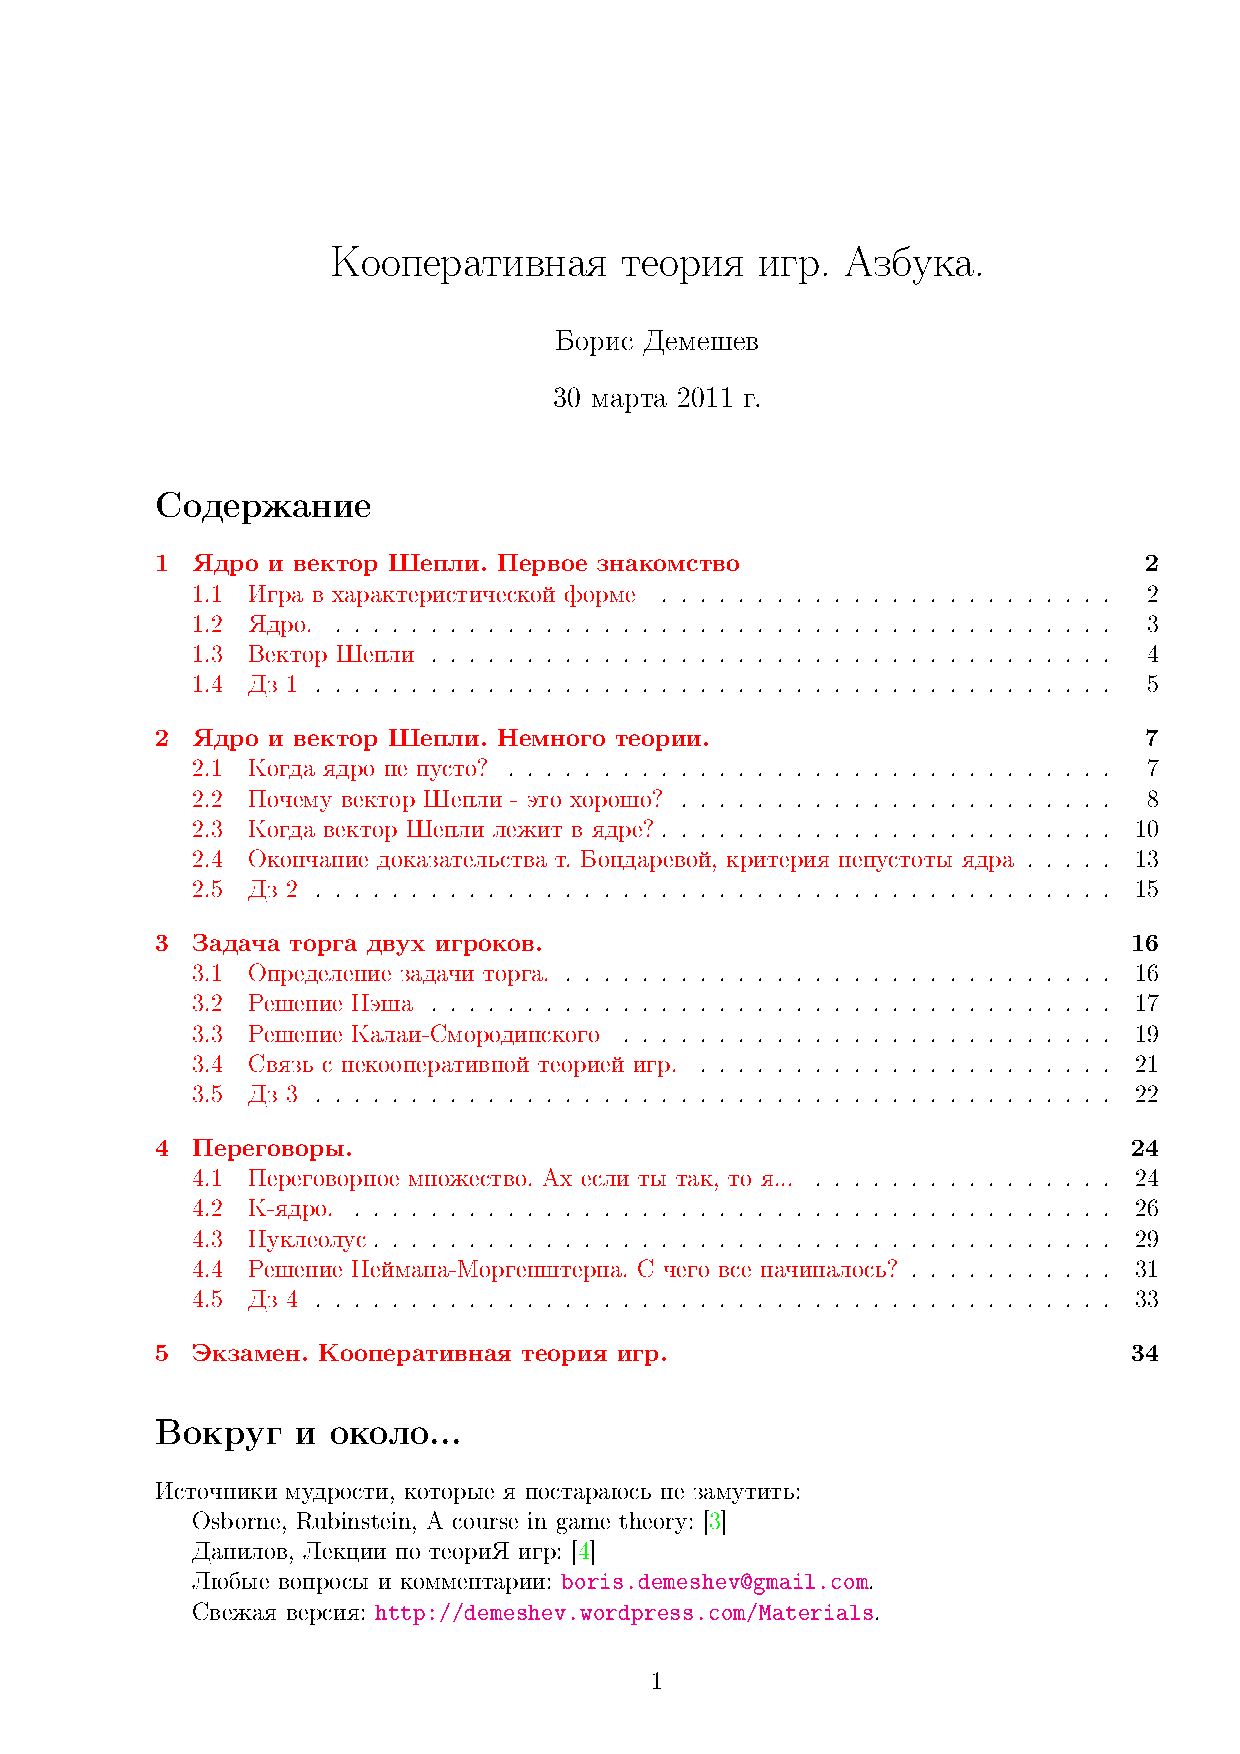
\includegraphics{coop_gt.3}
\end{figure}




\subsection{Окончание доказательства т. Бондаревой, критерия непустоты ядра}

Напомним формулировку:
\begin{theorem} $[$Бондарева$]$.
Ядро игры в характеристической форме непусто, если и только если для любого сбалансированного набора $\lambda_{S}$:
\begin{equation}
\label{balanced_game}
\sum_{S} \lambda_{S}v(S)\leq v(N)
\end{equation}
\end{theorem}

\begin{proof}


Обратно. Пусть неравенство \ref{balanced_game} выполнено.

Может есть какое-то более геометрическое\footnote{У Данилова в \cite{danilov:lte} через т. Какутани. Приведенное доказательство взято из Osborne, Rubinstein, \cite{osborne:cgt}} доказательство?

Для доказательства в обратную сторону нам понадобится технических факт:
\begin{theorem}
Два выпуклых множества в $R^{n}$ можно разделить гиперплоскостью. 
\end{theorem}
Этот факт мы примем без доказательства как хорошо согласующийся с геометрическими представлениями.

Введем обозначение $1_{S}$ - это вектор из $n$ чисел, каждое из которых равно нулю или единице, в зависимости от того, входит ли соответствующий участник в коалицию $S$. В частности, $1_{N}$ - это вектор из $n$ единичек, а $1_{\emptyset}$ - это вектор из $n$ нулей. Например, если $N=\{A,B,C,D\}$ и коалиция $S=\{A,D\}$, то $1_{S}=(1,0,0,1)$.

Вектор $1_{S}$ лежит в $n$-мерном пространстве.

Допишем к вектору $1_{S}$ стоимость соответствующей коалиции, получим вектор $(1_{S},v(S))$, лежащий в $(N+1)$-мерном пространстве.

Рассмотрим два множества (в $R^{n+1}$):

$A=\{(1_{N},v(N)+\varepsilon)| \varepsilon>0\}$. Это множество выпуклое, т.к. это полупрямая с выколотым началом.

$B=\{\sum_{S} \lambda_{S} (1_{S},v(S)) | \forall S \lambda_{S}\in [0;1] \}$. Это множество также выпуклое, т.к. является линейной комбинацией конечного числа векторов с произвольными неотрицательными весами. 

Эти множества не имеют общих точек, в силу неравенства \ref{balanced_game}. Оба множества выпуклы, значит существует гиперплоскость разделяющая множества $A$ и $B$.

Как существование такой гиперплоскости записать математически?

Это означает, что существует такой ненулевой вектор $\vec{\alpha}=(\alpha_{1},\alpha_{2},...,\alpha_{n+1})$, что:

\begin{equation}
\label{hyperplane_eq}
	\vec{\alpha}\cdot b \geq 0 > \vec{\alpha}\cdot a
\end{equation},
для любых $a\in A$ и $b\in B$.

Сначала мы докажем, что $\alpha_{n+1}<0$, а затем построим из $(\alpha_{1},\alpha_{2},...,\alpha_{n})$ элемент ядра.

Заметим, что $\alpha_{n+1}$ не может быть положительным: если бы оно было положительным можно было бы взять вектор $a$ с большим $\varepsilon$ и добиться положительности $\vec{\alpha}\cdot a$.

Уточним, что $\alpha_{n+1}$ не может быть равен нулю. Для этого рассмотрим вектор $v=(1_{N},v(N))$, начало полупрямой $A$. Он лежит в множестве $B$ - достаточно взять $\lambda_{N}=1$, а остальные $\lambda_{S}=0$. Поскольку вектор $v$ попадает на границу $A$ для него неравенство выглядит так: $\vec{\alpha}\cdot v \geq 0 \geq \vec{\alpha}\cdot v$.

Заметим, что $\vec{\alpha}\cdot v=\sum_{i=1}^{N}\alpha_{i}+\alpha_{n+1}v(N)$.

При $\alpha_{n+1}$ равном нулю мы получали бы, что $\sum_{i=1}^{n}\alpha_{i}=0$. Но это невозможно, т.к. в этом случае $\vec{\alpha}\cdot a$ равнялось бы нулю.

Маленький итог: $\alpha_{n+1}<0$. Значит неравенство \ref{hyperplane_eq} можно разделить на $(-\alpha_{n+1})$. При этом знаки неравенства не поменяются, а последняя компонента вектора $\vec{\alpha}$ превратится в минус единицу. Обозначим: $x_{i}=-\alpha_{i}/\alpha_{n+1}$.

Что это нам дает?

Левая часть неравенства говорит: для любого $b$: $(x_{1},x_{2},...,x_{n},-1)\cdot b \geq 0$.

Возьмем $b=(1_{S},v(S))$. Получаем, $\sum_{i\in S}x_{i}\geq v(S)$.

Правая часть неравенства говорит: для любого $a$: $(x_{1},x_{2},...,x_{n},-1)\cdot a <0$.

Возьмем $v=(1_{N},v(N))$. Этот вектор в $A$ не входит, но лежит на границе $A$, поэтому неравенство будет нестрогим: $\sum_{i\in N}x_{i}\leq v(N)$.

Что это значит? Это означает, что есть такой вектор $x$, который большая коалиция может выплатить (может у нее даже что-то останется). При этом ни одна коалиция $S$ не может получить больше, чем достается ей при дележе $x$. Следовательно, ядро не пусто.

\end{proof}










\end{document}